\documentclass{beamer}
\usetheme[style=plain]{uu}

\usepackage{graphicx}
\usepackage{mathtools}
\usepackage{amssymb}
\usepackage{hyperref}
\usepackage{color}
\usepackage{float}

%% unicode support, for text and code :)
\usepackage[utf8x]{inputenc}
\usepackage{ucs}
\usepackage{autofe}


%% Haskell syntax highlighting and code font
\usepackage{minted}
\usepackage{fancyvrb}
\usepackage{inconsolata}
\usemintedstyle{default}

\newmint{haskell}{mathescape,fontfamily=tt,fontsize=\footnotesize}
\newmintedfile{haskell}{xleftmargin=20pt,mathescape,fontfamily=tt,fontsize=\footnotesize}

\newminted{haskell}{xleftmargin=20pt,gobble=8,mathescape,fontfamily=tt,fontsize=\footnotesize}
\newmint{coq}{mathescape,fontfamily=tt,fontsize=\footnotesize}

\newmintedfile{coq}{xleftmargin=20pt,mathescape,fontfamily=tt,fontsize=\footnotesize}
\newminted{coq}{gxleftmargin=20pt,obble=8,mathescape,fontfamily=tt,fontsize=\footnotesize}



%% Metainformation
%% PDF stuff
\usepackage{datetime}
\usepackage{ifpdf}
\ifpdf
\pdfinfo{
    /Author (Joao Paulo Pizani Flor)
    /Title (Comparing functional EDSLs for hardware description)
    /Keywords (Hardware verification, Functional Programming, Hardware design, Dependently-typed programming, Coq, Lava, ForSyDe, Haskell, Coquet)
    /CreationDate (D:\pdfdate)
}
\fi

\title[Comparing functional EDSLs for hardware description]{Comparing functional Embedded Domain-Specific Languages for hardware description}

\date{February 13th, 2014}

\author[Pizani Flor]
{
    João Paulo Pizani Flor
}

\institute[Utrecht University]
{
    Department of Information and Computing Sciences,
    Utrecht University
}

\subject{Function Programming, Hardware verification, Haskell, Coq, Lava, Coquet, ForSyDe}




\begin{document}

%% The document itself
    \begin{frame}
        \titlepage
    \end{frame}

    \begin{frame}
        \frametitle{Table of Contents}
        \tableofcontents
    \end{frame}



    \section{Introduction}
    \label{sec:introduction}
        \frame{\sectionpage}

        \subsection{Hardware design}
        \label{subsec:hardware-design}
            \begin{frame}
                \frametitle{Hardware design}
            \end{frame}


        \subsection{Domain-Specific Languages}
        \label{subsec:domain-specific-languages}
            % deep-embedded / shallow embedded
            \begin{frame}
                \frametitle{Domain-Specific Languages}

                \par{A computer language (turing-complete or \emph{not}) targeting a \emph{specific application domain.}}
                \par{\textbf{Example DSLs:}}
                \begin{itemize}
                    \item SQL (database queries)
                    \item CSS (document formatting)
                    \item MATLAB (Matrix programming)
                    \item VHDL (Hardware description)
                \end{itemize}

                \pause

                \par{A DSL can also be \emph{embedded} in a general-purpose language.}
                \par{\textbf{Example EDSLs:}}
                \begin{itemize}
                    \item Boost.Proto (C++ / parser combinators)
                    \item Diagrams (Haskell / programmatic drawing)
                    \item Parsec (Haskell / parser combinators)
                \end{itemize}
            \end{frame}

            \begin{frame}[fragile]
                \frametitle{Example of an EDSL: \texttt{Parsec}}

                A simple parser for a "Game of Life"-like input format:
                \haskellfile{code/parsec-example.hs}
\end{frame}


        \subsection{Hardware EDSLs}
        \label{subsec:hardware-edsls}
            \begin{frame}
                \frametitle{Hardware EDSLs}
                An EDSL used for hardware design-related tasks. Can encompass:

                \begin{itemize}
                    \item Modelling / description
                    \item Simulation (validation)
                    \item Formal verification
                    \item Synthesis to other (lower-level) languages
                \end{itemize}
            \end{frame}

            \begin{frame}
                \frametitle{Example of a hardware EDSL}

                Some Lava code\ldots
            \end{frame}



    \section{Analyzed EDSLs}
    \label{sec:analyzed-edsls}
        \frame{\sectionpage}

        \subsection{Choice criteria}
        \label{subsec:edsls-choice-criteria}
            \begin{frame}
                \frametitle{Choice criteria}
            \end{frame}


        \subsection{Chosen EDSLs}
        \label{subsec:chosen-edsls}
            \begin{frame}
                \frametitle{Chosen EDSLs}
                The language we chose to evaluate, with the respective host language, were:

                \begin{itemize}
                    \item Lava (Haskell - \texttt{chalmers-lava} \emph{dialect})
                    \item ForSyDe (Haskell)
                    \item Coquet (Coq interactive theorem prover)
                \end{itemize}
            \end{frame}

        \subsection{Evaluation criteria}
        \label{subsec:evaluation-criteria}
            \begin{frame}
                \frametitle{Evaluation criteria}

                \begin{itemize}
                    \item Simulation
                    \item Verification
                    \item Genericity
                    \item Depth of embedding
                    \item Tool integration
                    \item Extensibility
                \end{itemize}
            \end{frame}



    \section{Modeled Circuits}
    \label{sec:modeled-circuits}
        \frame{\sectionpage}

        \subsection{Choice}
        \label{subsec:circuit-choice-criteria}
            \begin{frame}
                \frametitle{Choice criteria}

                \begin{itemize}
                    \item Not too simple, not too complex
                    \item Familiar to any hardware designer
                        \begin{itemize}
                            \item No signal processing, etc.
                        \end{itemize}
                    \item Well-defined, pre-specification
                        \begin{itemize}
                            \item Results to verify the models against
                        \end{itemize}
                \end{itemize}
            \end{frame}

            \begin{frame}
                \frametitle{Chosen circuits}

                \par{We cherry-picked circuits from the book ``Elements of Computing Systems'',
                    as they satisfied all of our demands.}

                \begin{figure}[h!]
                    \includegraphics[width=0.5\textwidth]{imgs/book-cover-elements.jpg}
                    \caption{``Elements of Computing Systems'' - Nisan, Schocken, \newline
                        available at \url{http://www.nand2tetris.org}.
                        \label{fig:book-cover-elements}
                    }
                \end{figure}
            \end{frame}

            \begin{frame}
                \frametitle{Chosen circuits}

                \begin{description}
                    \item[Circuit 1] A 2-input, 16-bit-wide, simple ALU
                    \item[Circuit 2] A 64-word long, 16-bit wide memory block
                    \item[Circuit 3] An \emph{extremely} reduced instruction set CPU,
                        the \emph{Hack} CPU.
                \end{description}
                \vspace{0.05\textwidth}

                \par{Let's take a quick look at each of these circuit's specification\ldots}
            \end{frame}


        \subsection{ALU}
        \label{subsec:alu}
            \begin{frame}
                \frametitle{Circuit 1: ALU}

                \par{Some of the circuit's key characteristics:}

                \begin{itemize}
                    \item 2 \emph{operand inputs} and 1 \emph{operand output}, each 16-bit wide
                    \item 1 \emph{output flag}
                    \item Can execute 18 different \emph{functions}, among which:
                        \begin{itemize}
                            \item Addition, subtraction
                            \item Bitwise AND / OR
                            \item Constant outputs
                            \item Addition of constants to an operand
                            \item Sign inversion
                        \end{itemize}
                \end{itemize}
            \end{frame}

            \begin{frame}
                \frametitle{Circuit 1: block diagram}

                \begin{figure}[h!]
                    \centerline{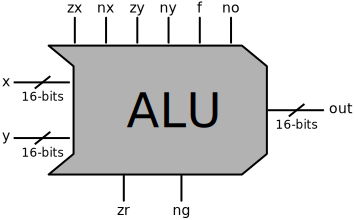
\includegraphics[width=0.6\textwidth]{imgs/alu-block.pdf}}
                    \caption{Input/Output ports of \emph{circuit 1}, the ALU.
                        \label{fig:alu-block}}
                \end{figure}
            \end{frame}

            \begin{frame}
                \frametitle{Circuit 1: specification}

                \par{The behaviour of the ALU is specified by the values of the \emph{control bits} and \emph{flags}:}

                \begin{description}
                    \item[\texttt{zx} and \texttt{zy}]
                        \emph{Zeroes} the ``\texttt{x}'' and ``\texttt{y}'' inputs, respectively
                    \item[\texttt{nx} and \texttt{ny}]
                        \emph{bitwise negation} on the ``\texttt{x}'' and ``\texttt{y}'' inputs
                    \item[\texttt{f}]
                        Selects the function to be applied: \newline
                        $\text{``\texttt{f}''} = 1$ for addition, $\text{``\texttt{f}''} = 0$ for bitwise AND
                    \item[\texttt{no}]
                        \emph{bitwise negation} on the output ALU output
                    \item[\texttt{zr} and \texttt{ng}]
                        The output \emph{flag} $\text{``\texttt{zr}''} = 1$ \emph{iff} the ALU output is zero.
                        $\text{``\texttt{ng}''} = 1$ \emph{iff} the output is negative.
                \end{description}

                \par{Formal definition and test cases in the book.}
            \end{frame}


        \subsection{Memory bank}
        \label{subsec:memory-bank}
            \begin{frame}
                \frametitle{Circuit 2: RAM64}

                \par{Some of the circuit's key characteristics:}

                \begin{itemize}
                    \item \emph{Sequential} circuit, with clock input
                    \item 64 memory words stored, each 16-bit wide
                    \item Address port has width $\log_{2} 64 = 6$ bit
                \end{itemize}
            \end{frame}

            \begin{frame}
                \frametitle{Circuit 2: block diagram}

                \begin{figure}[h!]
                    \centerline{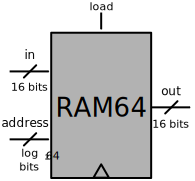
\includegraphics[width=0.45\textwidth]{imgs/ram-block.pdf}}
                    \caption{Input/Output ports of \emph{circuit 2}, the RAM64 block.
                        \label{fig:ram-block}}
                \end{figure}
            \end{frame}

            \begin{frame}
                \frametitle{Circuit 2: specification}

                \begin{itemize}
                    \item The output ``\texttt{out}'' holds the value at the memory line indicated by ``\texttt{address}''.
                    \item \emph{Iff} $\text{``\texttt{load}''} = 1$,
                        then the value at input ``\texttt{in}'' will be loaded into memory line ``\texttt{address}''.
                    \item The loaded value will be emitted on ``\texttt{out}'' at the \emph{next} clock cycle.
                \end{itemize}
            \end{frame}


        \subsection{CPU}
        \label{subsec:cpu}
            \begin{frame}
                \frametitle{Circuit 3: Hack CPU}

                \begin{itemize}
                    \item A \emph{very} reduced instruction set CPU
                        \begin{itemize}
                            \item Only 2 instructions: ``\texttt{C}'' and ``\texttt{A}''
                        \end{itemize}
                    \item Follows the \emph{Harvard architecture}
                        \begin{itemize}
                            \item Separate address spaces for \emph{data} and \emph{instruction} memory.
                        \end{itemize}
                    \item Instructions are 16-bits wide
                        \begin{itemize}
                            \item As well as the memory input and output
                        \end{itemize}
                    \item Two \emph{internal} registers: ``\texttt{D}'' and ``\texttt{A}''
                \end{itemize}
            \end{frame}

            \begin{frame}
                \frametitle{Circuit 3: block diagram}

                \begin{figure}[h!]
                    \centerline{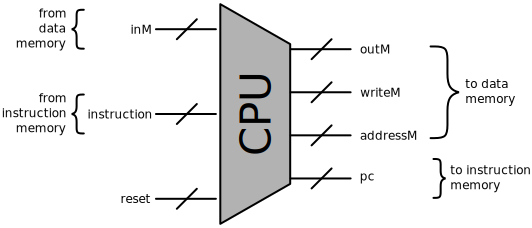
\includegraphics[width=1.0\textwidth]{imgs/cpu-block.pdf}}
                    \caption{Input/Output ports of \emph{circuit 3}, the \emph{Hack} CPU.
                        \label{fig:cpu-block}}
                \end{figure}
            \end{frame}

            \begin{frame}
                \frametitle{Circuit 3: specification}

                \par{Circuit 3 runs ``\texttt{A}'' and ``\texttt{C}'' instructions,
                according to the \emph{Hack assembly specification}.}

                \begin{itemize}
                    \item The ``\texttt{A}'' instruction: sets the ``\texttt{A}'' register.
                        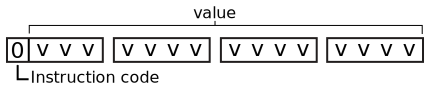
\includegraphics[width=0.8\textwidth]{imgs/cpu-instruction-a.pdf}
                    \vspace{0.5cm}
                    \item The value in ``\texttt{A}'' can be used:
                        \begin{itemize}
                            \item As operand for a subsequent computation
                            \item As address for jumps
                        \end{itemize}
                \end{itemize}
            \end{frame}

            \begin{frame}
                \frametitle{Circuit 3: specification}

                \par{Circuit 3 runs ``\texttt{A}'' and ``\texttt{C}'' instructions,
                according to the \emph{Hack assembly specification}.}

                \begin{itemize}
                    \item The ``\texttt{C}'' instruction:
                        sets the ``\texttt{C}'' register, performs \emph{computation} or jumps.
                        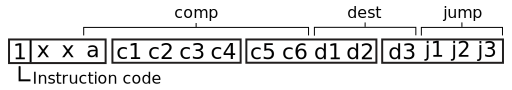
\includegraphics[width=0.85\textwidth]{imgs/cpu-instruction-c.pdf}
                    \vspace{0.5cm}
                    \item Some peculiarities:
                        \begin{itemize}
                            \item Bits ``\texttt{c1}'' to ``\texttt{c6}'' control the ALU
                            \item \emph{conditional} or \emph{unconditional} jumps
                            \item \emph{destination} of the computation result: ``\texttt{A}'', ``\texttt{D}'', ``\texttt{M}''
                        \end{itemize}
                \end{itemize}
            \end{frame}

            \begin{frame}
                \frametitle{Circuit 3: specification (parts)}

                \begin{figure}[h!]
                    \centerline{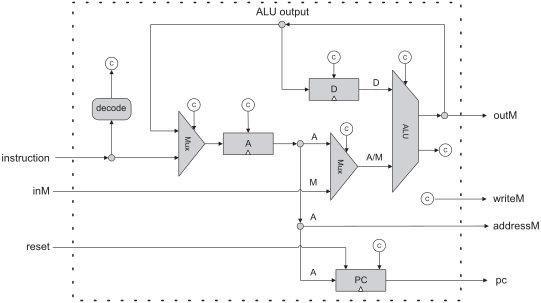
\includegraphics[width=1.05\textwidth]{imgs/cpu-parts.pdf}}
                    \caption{Parts used to build the \emph{Hack} CPU, and their interconnection.
                        \label{fig:cpu-parts}}
                \end{figure}
            \end{frame}



    \section{Analysis of the EDSLs}
    \label{sec:analysis-of-the-edsls}
        \frame{\sectionpage}

        \subsection{Lava}
        \label{subsec:lava}
            % Lava intro

            \begin{frame}
                \frametitle{Lava: Adders}
                \haskellfile{code/lava-adders.hs}
            \end{frame}

            \begin{frame}
                \frametitle{Lava: Simulation and verification}

                \begin{itemize}
                    \item A taste of simulation in Lava:
                        \haskellfile{code/lava-simulation-halfadder.hs}
                        \begin{itemize}
                            \item Cannot be easily automated: equality of \texttt{Signal} is non-trivial
                        \end{itemize}

                    \item And verification\ldots
                        \haskellfile{code/lava-verify-fulladder-comm.hs}
                        \begin{itemize}
                            \item Used in conjunction with an external SAT solver (e.g. \emph{Satzoo})
                            \item Only verifies instances of \emph{specific size}
                        \end{itemize}
                \end{itemize}
            \end{frame}

            % Lava ALU
            \begin{frame}
                \frametitle{Lava: ALU}
                \haskellfile{code/lava-alu.hs}
            \end{frame}

            \begin{frame}
                \frametitle{Remarks}

                \begin{itemize}
                    \item Cannot introduce new, meaningful datatypes
                        \begin{itemize}
                            \item Only \texttt{Signal Bool} is synthesizable
                            \item Or tuples/lists thereof
                        \end{itemize}
                    \item Input/Output types have to be \emph{uncurried}
                    \item Weak type-safety over the inputs/outputs
                        \begin{itemize}
                            \item Working with tuples is tiresome and has limitations
                            \item Lists don't enforce \emph{size} constraints
                        \end{itemize}
                \end{itemize}
            \end{frame}

            % Lava RAM64
            \begin{frame}
                \frametitle{Lava: RAM64}
                \haskellfile{code/lava-ram64.hs}
            \end{frame}

            \begin{frame}
                \frametitle{Remarks}

                \par{Positive:}
                \begin{itemize}
                    \item Uses host language for binding (\texttt{let}/\texttt{where}) and recursion
                    \item Uses host language for structural combinators
                \end{itemize}

                \par{Negative:}
                \begin{itemize}
                    \item Again, weak type-safety of lists, can cause problems at simulation
                    \item \emph{No modularity} in the generated VHDL code.
                \end{itemize}
            \end{frame}

            % Lava CPU
            \begin{frame}
                \frametitle{Lava: \emph{Hack} CPU}
            \end{frame}

            \begin{frame}
                \frametitle{Remarks}

                \par{Could benefit from:}
                \begin{itemize}
                    \item Fixed-length vectors
                        \begin{itemize}
                            \item ForSyDe-style or with type-level naturals in recent GHC.
                        \end{itemize}
                \end{itemize}
            \end{frame}


        \subsection{ForSyDe}
        \label{subsec:forsyde}
            % ForSyDe intro

            % ForSyDe ALU non-synth
            \begin{frame}
                \frametitle{ForSyDe: ALU (non-synth)}
                \haskellfile{code/forsyde-alu-slide1.hs}
            \end{frame}

            \begin{frame}
                \frametitle{ForSyDe: ALU (non-synth)}
                \haskellfile{code/forsyde-alu-slide2.hs}
            \end{frame}

            % ForSyDe Simulation

            % ForSyDe ALU synth

            \begin{frame}
                \frametitle{ForSyDe: Muxes}
                %% both advantage and disadvantage of ForSyDe
                \haskellfile{code/forsyde-muxes.hs}
            \end{frame}

            % ForSyDe RAM64
            \begin{frame}
                \frametitle{ForSyDe: RAM64}
                \haskellfile{code/forsyde-ram64.hs}
            \end{frame}

            % ForSyDe CPU


        \subsection{Coquet}
        \label{subsec:coquet}
            \begin{frame}
                \frametitle{The \texttt{Circuit} type}
                \coqfile{code/coquet-circuit-type.v}
            \end{frame}

            \begin{frame}
                \frametitle{Coquet}
                \coqfile{code/coquet-halfadder.v}
            \end{frame}

            \begin{frame}
                \frametitle{Coquet}
                \coqfile{code/coquet-fulladder.v}
            \end{frame}

            % Meaning relation
            \begin{frame}
                \frametitle{Coquet: Meaning relation}
                \coqfile{code/coquet-meaning-relation.v}
            \end{frame}

            % Specification definitions
            \begin{frame}
                \frametitle{Coquet: Specification}
                \coqfile{code/coquet-realise-implement.v}
            \end{frame}

            % Adder proof (1)
            \begin{frame}
                \frametitle{Coquet: Correctness proofs}
                \coqfile{code/coquet-halfadder-proof.v}
            \end{frame}

            % How to do proofs in Coquet (tac, etc)
            \begin{frame}
                \frametitle{Coquet: How to prove correctness}
                \coqfile{code/coquet-tac.v}
                % rinvert: invert derivation of meaning relation, following structure of circuit.
                % realise_all: use the Implement and Realise classes as hints to transform goals.
                % unreify_all: get rid of iso's
                % destruct all boolean, then proof by case analysis, not so important.
            \end{frame}
            % Adder proof (2)



    \section{Conclusions}
    \label{sec:conclusions}
        \frame{\sectionpage}

        \subsection{Results}
        \label{subsec:results}
            \begin{frame}
                \frametitle{Results}
            \end{frame}


        \subsection{Future work}
        \label{subsec:future-work}
            \begin{frame}
                \frametitle{Future work}
            \end{frame}


        \begin{frame}[plain]
            \begin{center}
                \par{\Huge{Thank you!}}
                \vspace{2.0cm}
                \par{\Huge{Questions?}}
            \end{center}
        \end{frame}


\end{document}
